\section{System Outcomes and Enhancements}

\subsection{Achieved Performances}
Once the system features were delivered, a particular focus was made on the performances in order to mett the NFR6 (see \cref{tab:nfr}). This was possible through the usage of the Performance Monitoring tool provided by the Firebase platform.
\subsubsection{Startup Time}
The performance tool allowed to monitor the application startup time as main metric of relevance. The Firebase Performance library allowed an easy monitoring implementation by creating a \texttt{trace} instance, call his \texttt{start} method, perform the application startup and then call the \texttt{stop} method. The timespan considered was 60 days, the largest one allowed. The trend is declining, since the data fetch operations are called only for the shown data, and not for the whole dataset. However, it has to be said that peak values found were over 2 seconds: that was the case when the backup task severely impacted on the metric performances (\texttt{performLocalBackup} method, see \cref{subsec:backup}). In any case, the 90th percentile relative to the metric is 971 ms, so well under 2 seconds.

\begin{figure*}
    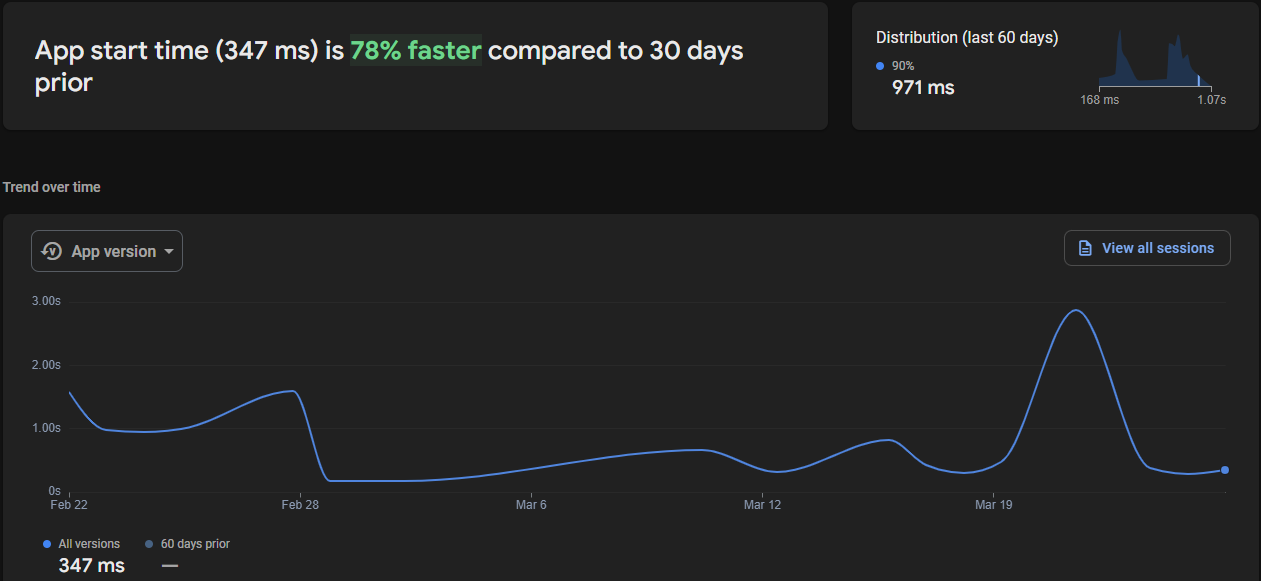
\includegraphics[width=1.0\linewidth]{./images/performance.png}
    \caption{Performance analysis of the startup time metric, with very good results.}
\end{figure*}
\newpage
\subsubsection{API Calls}
Also the API calls were monitored, in order to understand the impact of the data fetching operations on the overall performances. Also in this case the timespan considered was 60 days, and each API call was monitored with a \texttt{trace} object, like the application startup. Without focusing on a specific API, on average the results were pretty good, since we had an average response time of 176 ms and an increasing performance trend of the 25.48\%. 
\vspace{10ex}
\begin{figure*}
    \centering
    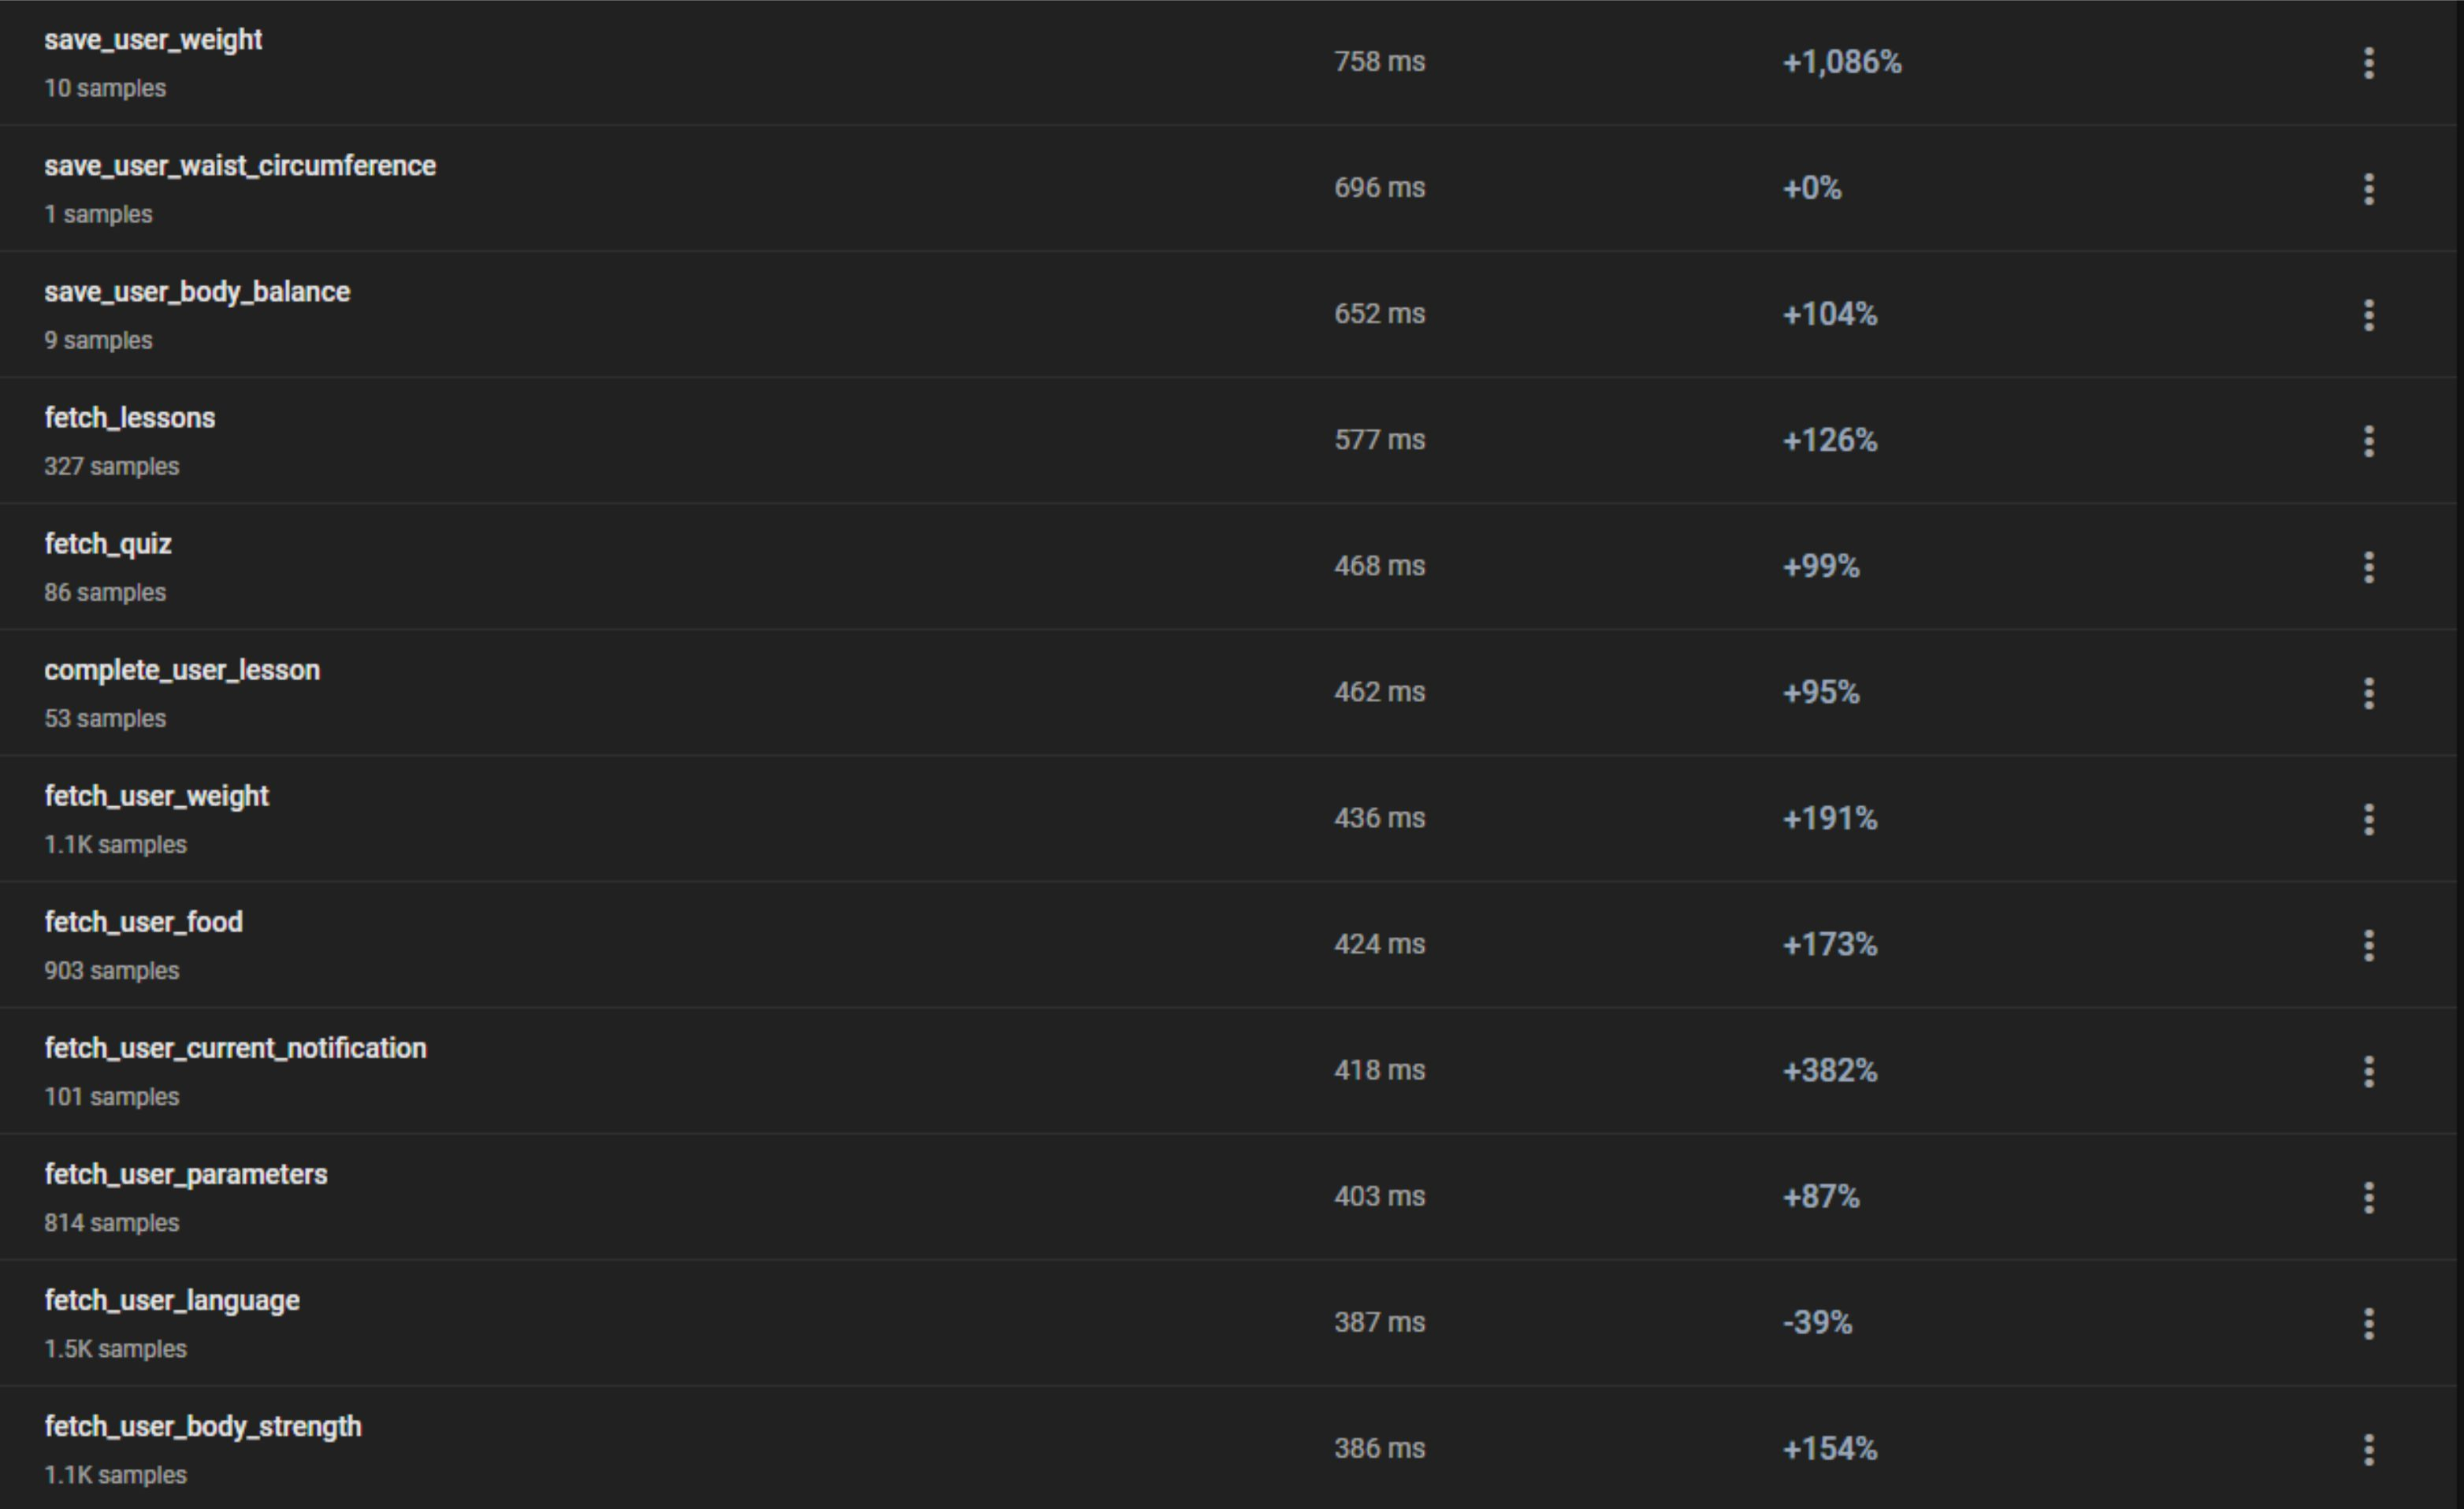
\includegraphics[width=0.8\linewidth]{./images/apiPerformances.jpg}
    \caption{Performance of the API calls.}
\end{figure*}

\begin{figure*}
    \centering
    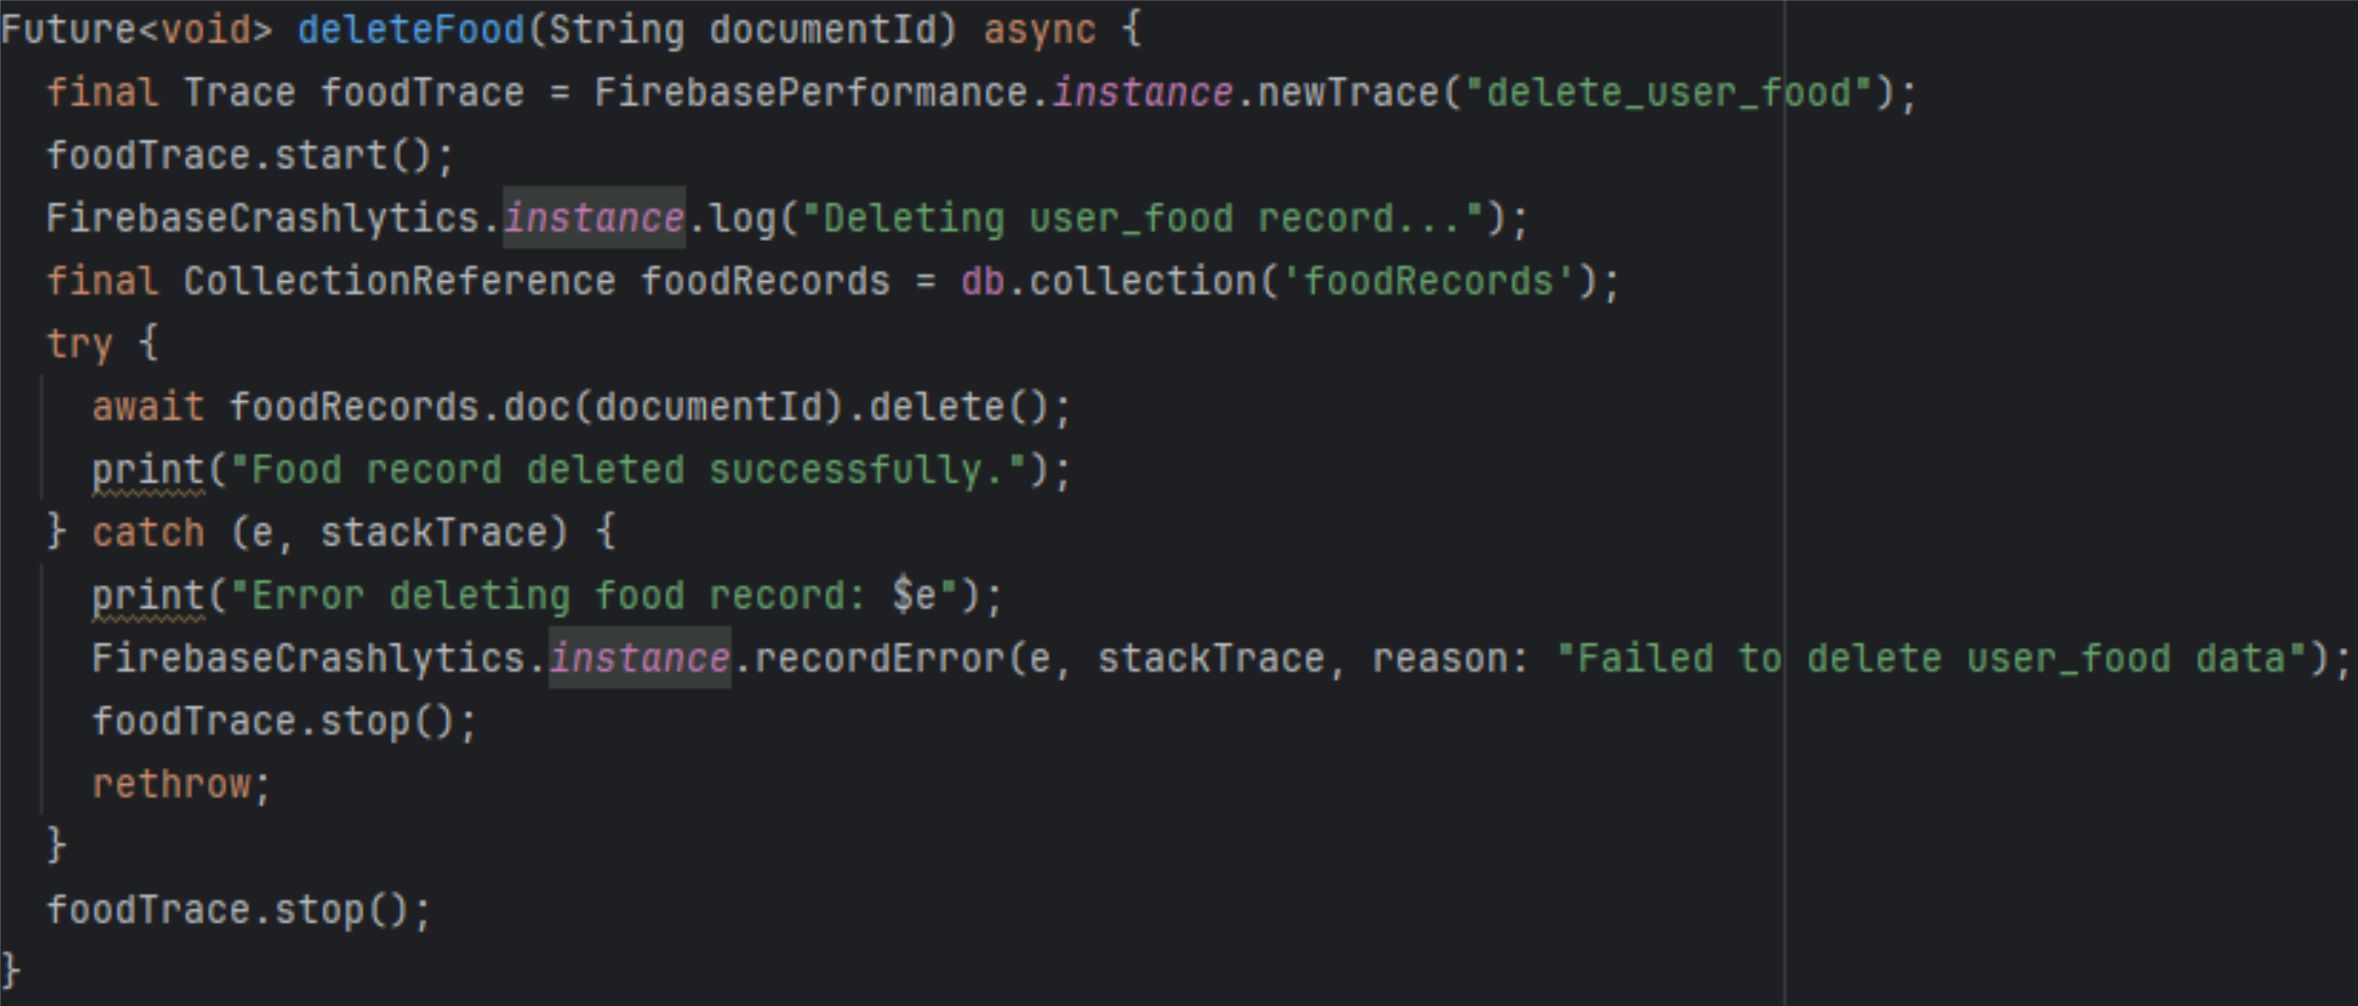
\includegraphics[width=0.8\linewidth]{./images/deleteFoodMonitoring.jpg}
    \caption{Monitoring example on the deleteFood API call.}
\end{figure*}
\newpage
\subsection{Crashlytics}
Also the \texttt{Crashlytics} tool has been helpful, thanks to the crash monitoring and the possibility to deeply analyze the log related to errors submitted. Thanks to this tool provided by the Firebase platform, a bug in the Health Data Backup (see \cref{subsec:backup}) was detected and fixed consequently. This allowed to improve the overall stability of the application, passing from a 93.7\% crash-free users to a 100\% crash-free users. Even though is not a big improvement and the percentage was already high, it still improved the overall system stability and worth to mention.
\vspace{10ex}
\begin{figure*}
    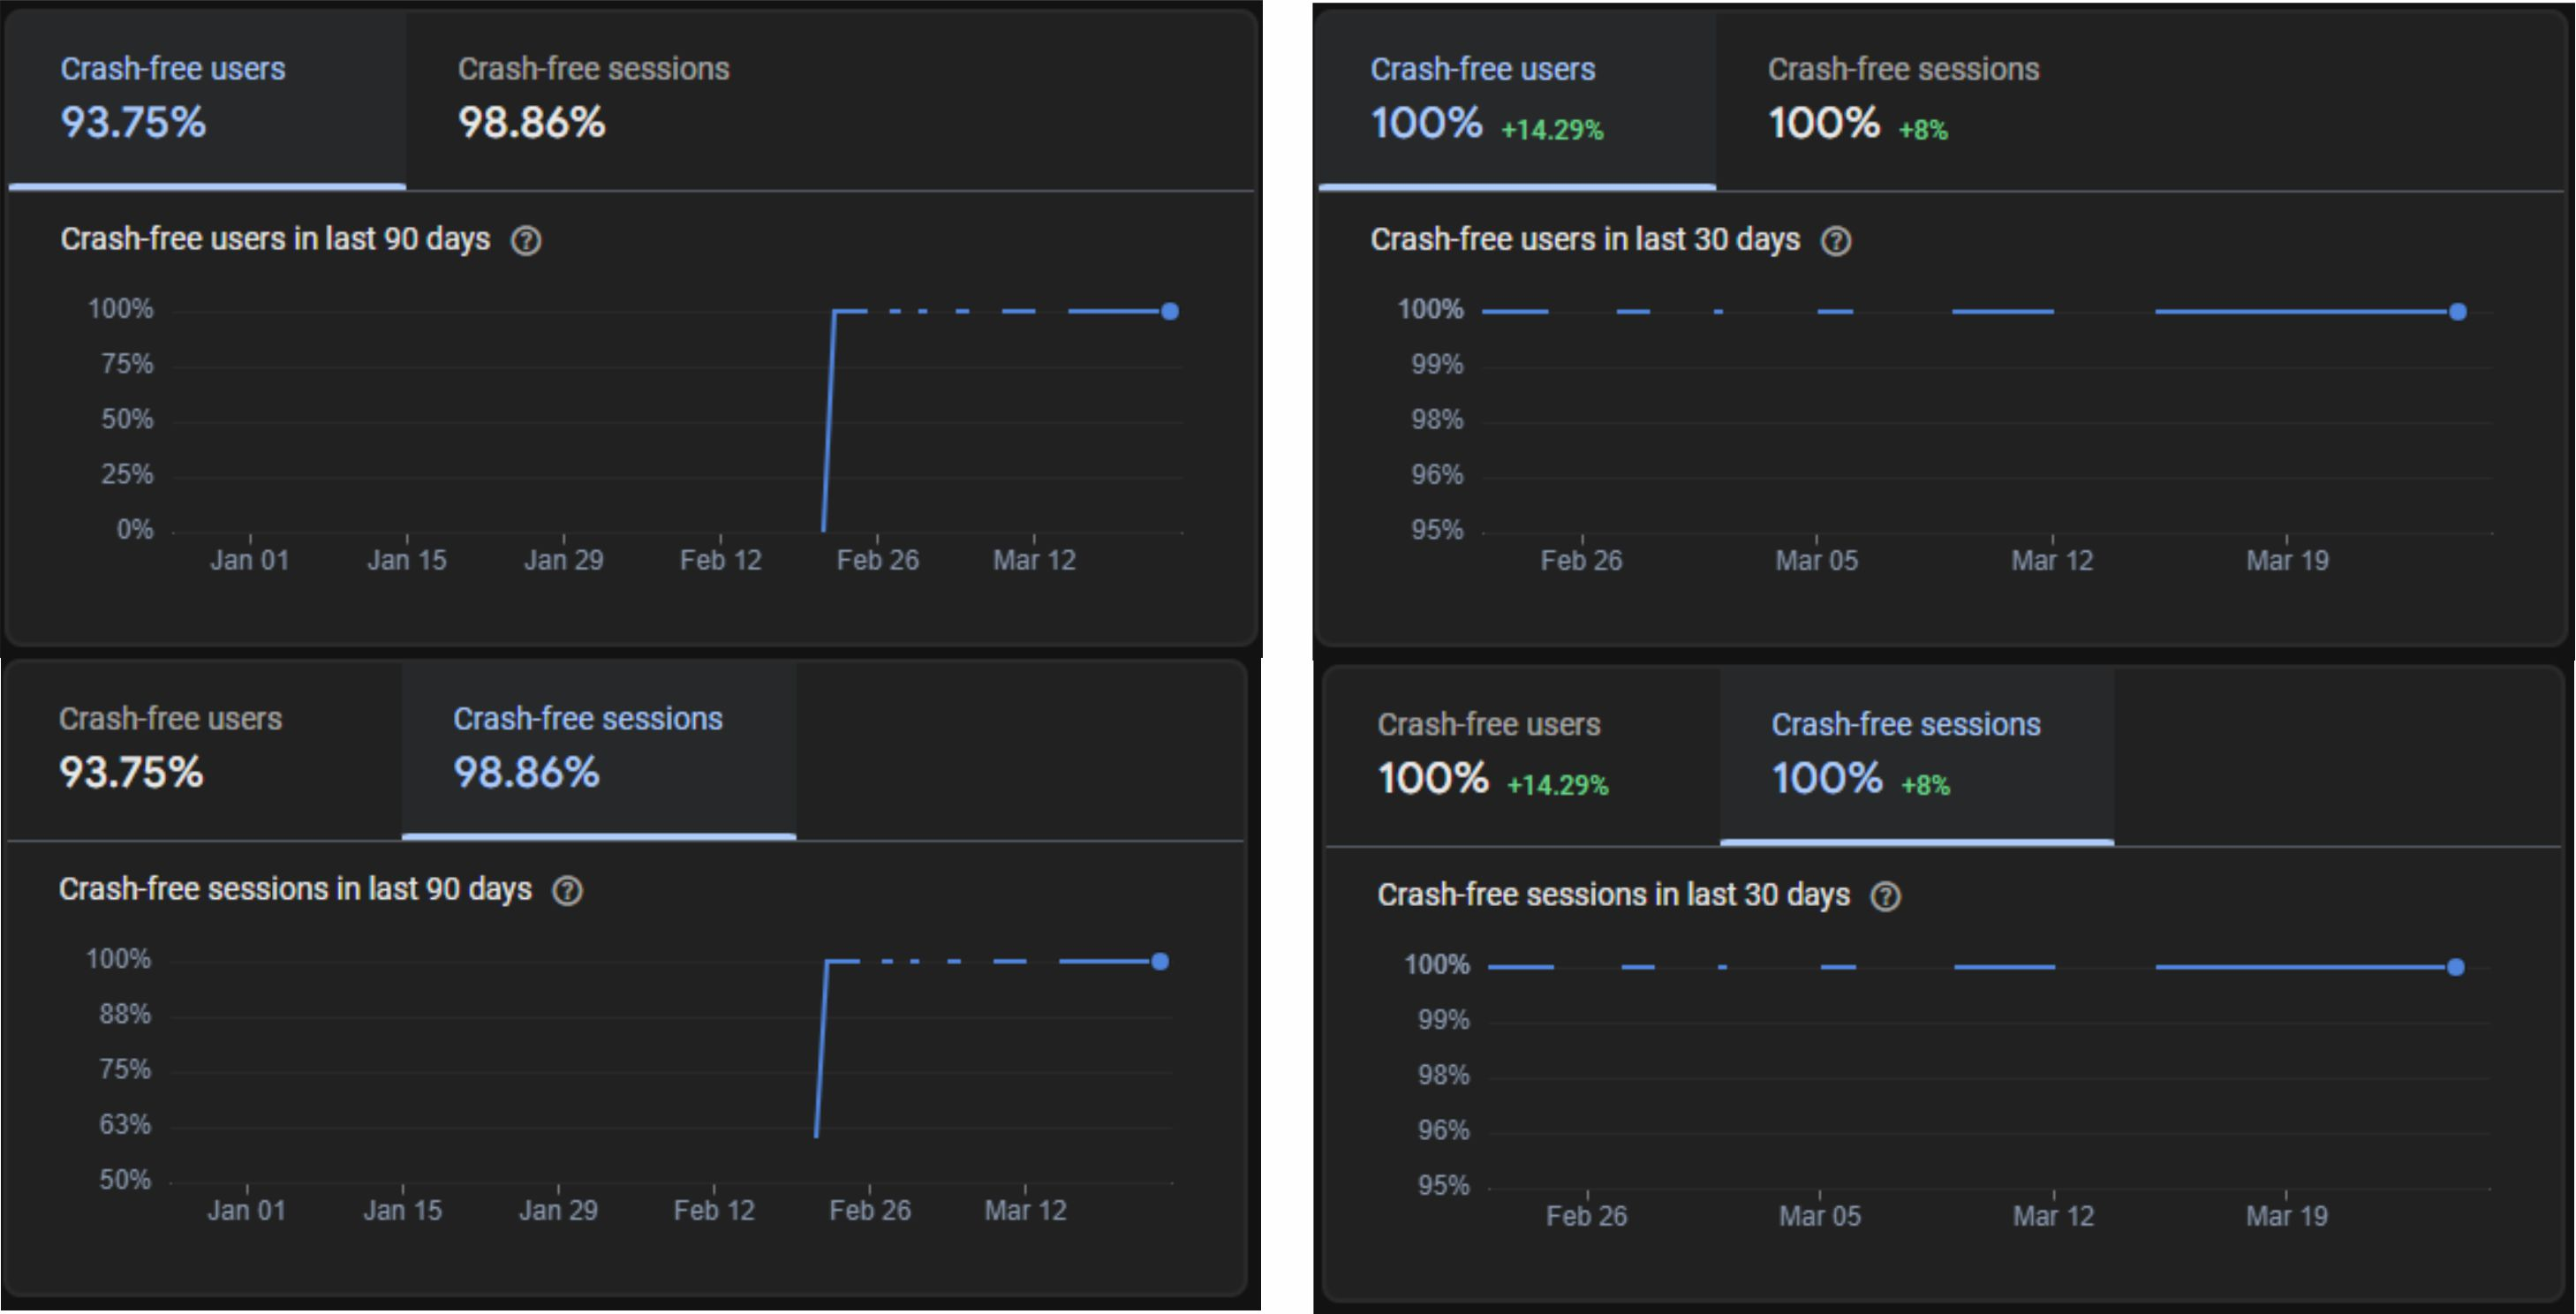
\includegraphics[width=1.0\linewidth]{./images/crashlytics.jpg}
    \caption{Crash-free users and session in the last 90 days, with the bug present (left) and in the last 30 datìys, after the bug fix (right).}
\end{figure*}

\newpage
\subsection{Future Developments}
Rarely a system can be considered perfect. There is always room for improvement in several aspects, so of course a future development can be done on this side.
\newline Having said that, other than improvement on current features, other possible new features have been considered in this system, that can definitely make it different, allowing to stand out from the competition. 

\begin{itemize}[nosep] % 'nosep' removes extra spacing between items
    \item \textbf{Ios Integration:} the system is designed to be intrisecely cross-platform from a smartphone point of view (since flutter is cross-platform and supports IOS). For this reason, from a theoretically point of view, the IOS support shouls already be present in the system. However, the system has not been tested practically on IOS devices, since a mac, IOS device and an apple watch are needed to test the system in its entirety, and these devices were not in our possession. For this reason IOS was not covered in the elaborate and should be tested to assess the effective cross-platform support.
    \item \textbf{Personal Coach:} integrate another component in the system architecture acting as a personal coach by generating personalized health and fitness recommendations. The goal would be to provide data-driven, actionable, and behavior-changing insights tailored to the user. This would be possible thanks to the integration of a Large Language Model (LLM) that can generate personalized recommendations based on the user's data. In fact, the backup feature already present and integrated into the system has been developed precisely to allow this data to be used in the LLM model in order to provide user-tailored insights and guaranteee the best user experience possible.
    \item \textbf{Personal Coach App Integration:} once developed and deployed the personal coach, there would be the integration inside the application: infact, this should be the purpose of the recommend page (reachable through the central button in the bottom navigation bar), that has been added to the app, in addition to the home, health measures, personal information and learn pages. This page will be used to integrate the LLM model in the future, by inserting some recommendations generated by the model. It would also be useful to have the possibility to chat with the personal coach, in order to ask for clarifications or to have more information about the recommendations provided.
\end{itemize}